\documentclass[12pt,a4paper]{article}

% ---------------- Packages ----------------
\usepackage[a4paper,margin=1in]{geometry}
\usepackage{graphicx}
\usepackage{setspace}
\usepackage{array}
\usepackage{longtable}
\usepackage{fancyhdr}
\usepackage{titlesec}
\usepackage[hidelinks]{hyperref}
\usepackage[normalem]{ulem}
\usepackage{xurl}
\usepackage{amsmath}
\usepackage{tikz}
\usepackage{everypage}
\usetikzlibrary{calc,arrows.meta,positioning} 

% -------- Page Borders --------
\AddEverypageHook{
\begin{tikzpicture}[remember picture,overlay]
\draw[line width=1pt]
    ($(current page.north west)+(1cm,-1cm)$)
    rectangle
    ($(current page.south east)+(-1cm,1cm)$);
\end{tikzpicture}
}

% -------- Font --------
\usepackage{newtxtext,newtxmath}

% ---------------- Spacing ----------------
\setstretch{1.5}
\setlength{\parindent}{0pt}

% ---------------- Section Style ----------------
\titleformat{\section}
  {\bfseries\large}
  {\thesection}
  {0.3cm}
  {}

% ---------------- Footer ----------------
\pagestyle{fancy}
\fancyhf{}
\fancyfoot[C]{\thepage\ | Page}

% =================================================
\begin{document}

% ================= TITLE PAGE ====================
\thispagestyle{empty}

\vspace*{-1.5cm}

\begin{center}
% Note: Ensure you have a 'media' folder with 'logo.png' in the same directory, 
% or comment out the next line if you don't have the image file yet.
\IfFileExists{media/logo.png}{\includegraphics[width=10cm]{media/logo.png}}{\vspace*{2cm}} 
\end{center}

\vspace{0.15cm}

\begin{center}
{School of Computer Science and Engineering} \\
\vspace{0.15cm}
{B. Tech COMPUTER SCIENCE ENGINEERING - ARTIFICIAL INTELLIGENCE AND MACHINE LEARNING} \\
\vspace{0.15cm}
\uline{\textbf{Statistics and Probability }} \\
\vspace{0.15cm}
\uline{\textbf{(25BSMAO4)}} \\
\vspace{0.5cm}
\textbf{\underline{EXPERIENTIAL LEARNING ON :-}} \\
\vspace{0.2cm}
\textbf{\underline{Household Energy Consumption Analysis}}
\end{center}

\vspace{0.15cm}



\begin{center}
\begin{center}
{Submitted to}
\end{center}
\textbf{Prof. Vishwanatha S,} \\
Assistant Professor, \\
Department of Mathematics, \\
Faculty of Engineering \& Technology, \\
Jain (Deemed-to-be) University.
\end{center}


% -------- Submitted By Table --------
\begin{center}
{Submitted by}
\end{center}
\renewcommand{\arraystretch}{1.1}
\begin{center}
\begin{tabular}{|p{4cm}|p{4cm}|p{6cm}|}
\hline
\textbf{USN} & \textbf{Name} & \textbf{Individual Contribution} \\
\hline
25BTRCL174 & Ojas Chaudhary & JavaScript analytics, dashboard integration, and project coordination \\
\hline
25BTRCL126 & Lakshmi Sinu Subhagan & Dataset review, statistical interpretation, and documentation support \\
\hline
25BTRCL130 & Lochana DN & HTML interface structure, data table review, and report section validation \\
\hline
25BTRCL170 & Nishtha Shankar & CSS styling, responsive layout review, and visual presentation refinement \\
\hline
25BTRCL175 & Omsai & Probability, hypothesis testing, simulation review, and inference checking \\
\hline
25BTRCL150 & Mishti & Report synthesis, conclusion drafting, and content consistency review \\
\hline
 &  &  \\
\hline
\end{tabular}
\end{center}


\newpage



\vspace{0.15cm}

% -------- Program / Date Table --------
\begin{center}
\begin{tabular}{|p{7cm}|>{\centering\arraybackslash}p{7cm}|}
\hline
\textbf{Program \& Section:} & B.Tech CSE-AIML 'C' \\
\hline
\textbf{Date of Submission:} & 13/04/2026 \\
\hline
\end{tabular}
\end{center}

\begin{center}
\begin{tabular}{|p{7cm}|>{\centering\arraybackslash}p{7cm}|}
\hline
\textbf{Total Marks:} &  \\
\hline
\textbf{Remarks} &  \\
\hline
\end{tabular}
\end{center}

% ================= INDEX ====================
\setcounter{page}{2}
\setcounter{section}{0}

\section*{INDEX}

\vspace{0.5cm}

\begin{center}
\begin{tabular}{|c|p{10cm}|c|}
\hline
\textbf{Sl.no.} & \textbf{Title} & \textbf{Page No.} \\
\hline
1 & \hyperref[sec:problem]{\textbf{Problem Statement}} & \pageref{sec:problem} \\
\hline
2 & \hyperref[sec:objective]{\textbf{Objectives}} & \pageref{sec:objective} \\
\hline
3 & \hyperref[sec:motivation]{\textbf{Motivation}} & \pageref{sec:motivation} \\
\hline
4 & \hyperref[sec:data]{\textbf{Data Source}} & \pageref{sec:data} \\
\hline
5 & \hyperref[sec:model]{\textbf{Mathematical Model (Data Usage and \mbox{Analysis)}}} & \pageref{sec:model} \\
\hline
6 & \hyperref[sec:code]{\textbf{Tool Based Approach (Code, Visual \mbox{Presentations}
and Interpretations}} & \pageref{sec:code} \\
\hline
7 & \hyperref[sec:simulation]{\textbf{Validation or Simulation (Reflection and
Critical Thinking)}} & \pageref{sec:simulation} \\
\hline
8 & \hyperref[sec:conclusion]{\textbf{Conclusions}} & \pageref{sec:conclusion} \\
\hline
9 & \hyperref[sec:appendix]{\textbf{Appendix: Raw Data and Calculations}} & \pageref{sec:appendix} \\
\hline
\end{tabular}
\end{center}

\newpage

% ================= CONTENT ====================

\section{Problem Statement}
\label{sec:problem}

Household electricity use is influenced by appliance operation, lighting use, indoor room conditions, and external weather factors. Since these variables change continuously over time, raw observations alone do not provide a clear understanding of consumption behavior. The problem addressed in this project is to analyze household energy consumption data and convert it into meaningful statistical information through descriptive analysis, probability estimation, relationship analysis, hypothesis-based comparison, and simulation.

The project implements an interactive web dashboard titled \textit{Household Energy Consumption Analysis}. It uses the local \texttt{data.csv} file and browser-based code to summarize appliance and lighting consumption patterns. The central question considered in the work is: how can statistical methods be used to describe, interpret, and simulate household appliance energy consumption from observed environmental and usage variables?

\section{Objectives}
\label{sec:objective}

\begin{enumerate}
\item To load and examine the Appliance Energy Prediction dataset containing household energy and environmental measurements.
\item To compute descriptive statistics such as mean, median, mode, variance, and standard deviation for selected variables.
\item To study the relationship between appliance energy consumption and lighting energy consumption using correlation and scatter visualization.
\item To estimate empirical probabilities for selected appliance and lighting consumption conditions.
\item To compare appliance consumption under different lighting levels through a hypothesis-based descriptive test.
\item To perform Monte Carlo style simulation for possible future values of appliance or lighting energy consumption.
\item To present the analysis through a responsive browser-based dashboard using HTML, CSS, JavaScript, and Chart.js.
\end{enumerate}




\section{Motivation}
\label{sec:motivation}

Energy consumption analysis is important for improving household efficiency, reducing unnecessary electricity usage, and understanding how daily activity patterns affect demand. Appliances usually represent a major part of household energy consumption, while lighting and indoor environmental conditions may indicate occupancy, behavior, and time-dependent usage patterns. Statistical analysis helps convert these observations into measurable insights.

This project is motivated by the need to connect classroom concepts from Statistics and Probability with a practical dataset. Measures of central tendency and dispersion describe normal and variable consumption behavior. Probability estimates quantify the likelihood of high-demand conditions. Correlation and graphical representations reveal relationships between variables, while simulation allows possible future patterns to be explored. The web dashboard format also makes the analysis interactive and easier to interpret for non-specialist users.

\section{Data Source)}
\label{sec:data}

The data source used in the project is the local file \texttt{data.csv}. The README identifies it as the Appliance Energy Prediction dataset used for household energy analysis. The CSV file contains 19,735 observations and 29 variables. Each observation is time stamped, and the local dataset ranges from \texttt{2016-01-11 17:00:00} to \texttt{2016-05-27 18:00:00}. Measurements are recorded at approximately 10-minute intervals.

The dataset contains the following main categories of variables:

\begin{itemize}
\item \textbf{Energy variables:} \texttt{Appliances} gives appliance energy consumption in Wh, and \texttt{lights} gives lighting energy consumption in Wh.
\item \textbf{Indoor temperature variables:} \texttt{T1} to \texttt{T9} represent temperature readings for different indoor zones.
\item \textbf{Indoor humidity variables:} \texttt{RH\_1} to \texttt{RH\_9} represent relative humidity readings for corresponding zones.
\item \textbf{Outdoor and weather variables:} \texttt{T\_out}, \texttt{RH\_out}, \texttt{Windspeed}, \texttt{Visibility}, \texttt{Press\_mm\_hg}, and \texttt{Tdewpoint} describe external weather conditions.
\item \textbf{Random variables:} \texttt{rv1} and \texttt{rv2} are additional random variables included in the dataset.
\end{itemize}

\begin{table}[htbp]
\centering
\caption{Summary of dataset variable groups used in the analysis}
\label{tab:dataset-variable-groups}
\begin{tabular}{|p{4cm}|p{8.5cm}|}
\hline
\textbf{Variable Group} & \textbf{Description} \\
\hline
Energy consumption & Appliance and lighting energy usage measured in Wh. \\
\hline
Indoor environment & Room-wise temperature and relative humidity measurements from zones 1 to 9. \\
\hline
Outdoor weather & Outdoor temperature, humidity, windspeed, visibility, pressure, and dew point. \\
\hline
Auxiliary variables & Random variables \texttt{rv1} and \texttt{rv2} included with the dataset. \\
\hline
\end{tabular}
\end{table}

No missing values were found in the columns of the local CSV file. The dashboard focuses mainly on \texttt{Appliances}, \texttt{lights}, \texttt{T1}, \texttt{RH\_1}, and \texttt{T\_out}, while the data table displays all available variables dynamically.

\section{Mathematical Model (Data Usage and Analysis)}
\label{sec:model}

Let $x_1, x_2, \ldots, x_n$ denote the observed values of a selected numerical variable. The dashboard applies the following statistical measures to analyze the dataset:

\[
\bar{x} = \frac{1}{n}\sum_{i=1}^{n}x_i
\]

\[
\sigma^2 = \frac{1}{n}\sum_{i=1}^{n}(x_i-\bar{x})^2, \qquad
\sigma = \sqrt{\sigma^2}
\]

The mean $\bar{x}$ describes average consumption, variance $\sigma^2$ measures spread, and standard deviation $\sigma$ expresses variability in the same unit as the original variable. The median and mode are also computed to identify the central and most frequent observed values.

For two variables $X$ and $Y$, the relationship is measured using Pearson correlation:

\[
r = \frac{\sum_{i=1}^{n}(x_i-\bar{x})(y_i-\bar{y})}
{\sqrt{\sum_{i=1}^{n}(x_i-\bar{x})^2}\sqrt{\sum_{i=1}^{n}(y_i-\bar{y})^2}}
\]

Empirical probability is calculated by counting the number of observations satisfying a condition and dividing it by the total number of observations:

\[
P(A)=\frac{\text{Number of observations satisfying condition } A}{\text{Total number of observations}}
\]

The local dataset produced the following selected descriptive results:

\begin{longtable}{|p{3.2cm}|p{2.2cm}|p{2.2cm}|p{2.2cm}|p{2.2cm}|}
\caption{Selected descriptive statistics computed from \texttt{data.csv}}
\label{tab:descriptive-statistics}\\
\hline
\textbf{Variable} & \textbf{Mean} & \textbf{Median} & \textbf{Std. Dev.} & \textbf{Range} \\
\hline
\texttt{Appliances} & 97.695 & 60.000 & 102.522 & 10 to 1080 \\
\hline
\texttt{lights} & 3.802 & 0.000 & 7.936 & 0 to 70 \\
\hline
\texttt{T1} & 21.687 & 21.600 & 1.606 & 16.79 to 26.26 \\
\hline
\texttt{RH\_1} & 40.260 & 39.657 & 3.979 & 27.023 to 63.360 \\
\hline
\texttt{T\_out} & 7.412 & 6.917 & 5.317 & -5 to 26.1 \\
\hline
\end{longtable}

The correlation between \texttt{Appliances} and \texttt{lights} is approximately 0.197. This indicates a positive but weak relationship: higher lighting consumption is associated with higher appliance consumption in some cases, but lighting alone does not fully explain appliance energy demand. The empirical probability that appliance consumption exceeds 100 Wh is approximately 21.45\%, while the probability that lighting consumption is 0 Wh is approximately 77.28\%.

\begin{figure}[htbp]
\centering
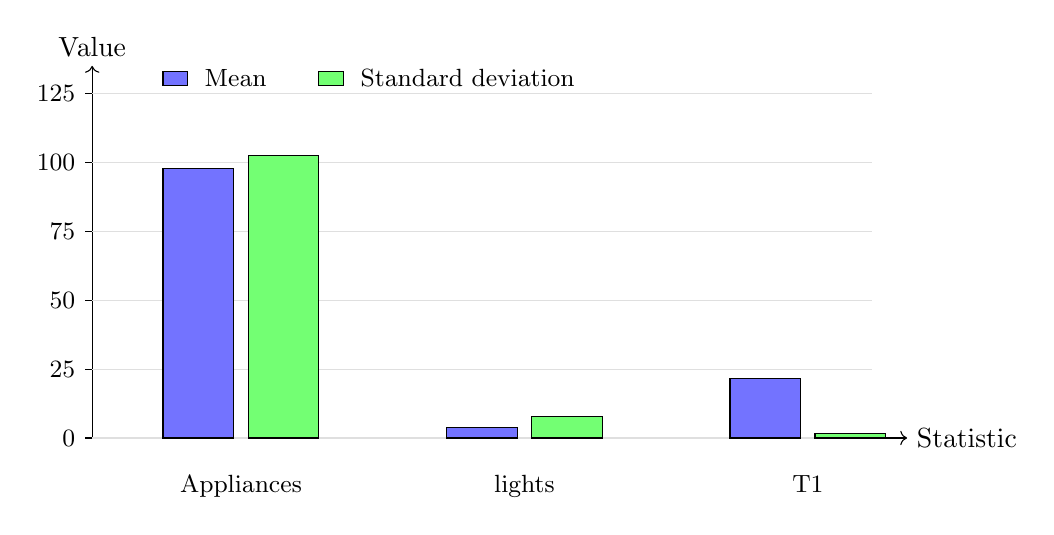
\begin{tikzpicture}[x=0.9cm,y=0.035cm]
\draw[->] (0,0) -- (11.5,0) node[right]{Statistic};
\draw[->] (0,0) -- (0,135) node[above]{Value};
\foreach \y in {0,25,50,75,100,125}
{
    \draw (-0.1,\y) -- (0,\y);
    \node[left] at (-0.1,\y) {\small \y};
    \draw[gray!25] (0,\y) -- (11,\y);
}
\draw[fill=blue!55] (1,0) rectangle (2,97.695);
\draw[fill=green!55] (2.2,0) rectangle (3.2,102.522);
\node[below,align=center] at (2.1,-10) {\small Appliances};
\draw[fill=blue!55] (5,0) rectangle (6,3.802);
\draw[fill=green!55] (6.2,0) rectangle (7.2,7.936);
\node[below,align=center] at (6.1,-10) {\small lights};
\draw[fill=blue!55] (9,0) rectangle (10,21.687);
\draw[fill=green!55] (10.2,0) rectangle (11.2,1.606);
\node[below,align=center] at (10.1,-10) {\small T1};
\draw[fill=blue!55] (1,128) rectangle (1.35,133);
\node[right] at (1.45,130.5) {\small Mean};
\draw[fill=green!55] (3.2,128) rectangle (3.55,133);
\node[right] at (3.65,130.5) {\small Standard deviation};
\end{tikzpicture}
\caption{Graph comparing mean and standard deviation for selected analysis variables}
\label{fig:descriptive-graph}
\end{figure}

\begin{figure}[htbp]
\centering
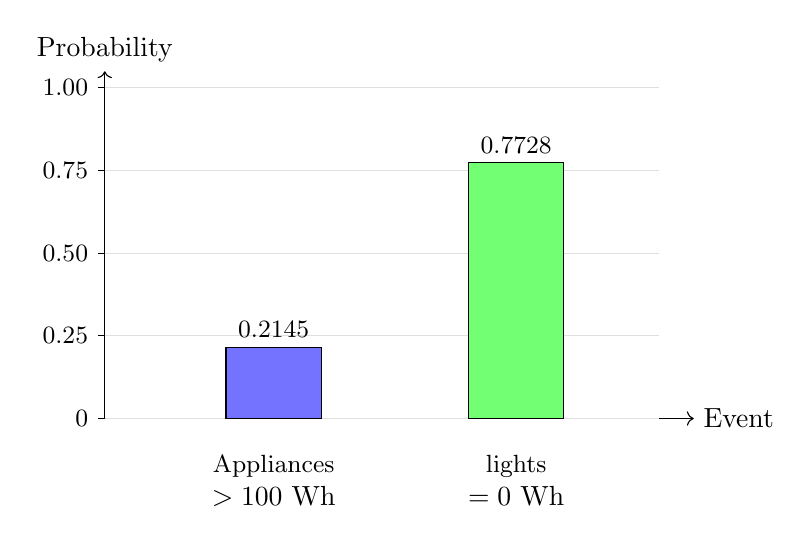
\begin{tikzpicture}[x=2.2cm,y=4.2cm]
\draw[->] (0,0) -- (3.4,0) node[right]{Event};
\draw[->] (0,0) -- (0,1.05) node[above]{Probability};
\foreach \y/\label in {0/0,0.25/0.25,0.5/0.50,0.75/0.75,1/1.00}
{
    \draw (-0.04,\y) -- (0,\y);
    \node[left] at (-0.04,\y) {\small \label};
    \draw[gray!25] (0,\y) -- (3.2,\y);
}
\draw[fill=blue!55] (0.7,0) rectangle (1.25,0.2145);
\node[below,align=center] at (0.975,-0.08) {\small Appliances\\$>100$ Wh};
\node[above] at (0.975,0.2145) {\small 0.2145};
\draw[fill=green!55] (2.1,0) rectangle (2.65,0.7728);
\node[below,align=center] at (2.375,-0.08) {\small lights\\$=0$ Wh};
\node[above] at (2.375,0.7728) {\small 0.7728};
\end{tikzpicture}
\caption{Graph of selected empirical probabilities from the dataset}
\label{fig:probability-graph}
\end{figure}

\section{Tool Based Approach (Code, Visual
Presentations
and Interpretations}
\label{sec:code}

The implementation uses a client-side web application composed of \texttt{index.html}, \texttt{style.css}, and \texttt{script.js}. The dashboard is organized into six tabbed sections: Overview, Dataset, Statistics, Inference, Simulation, and Report. The interface is built in HTML using semantic sections, tables, form controls, and Chart.js canvas elements.

\begin{figure}[htbp]
\centering
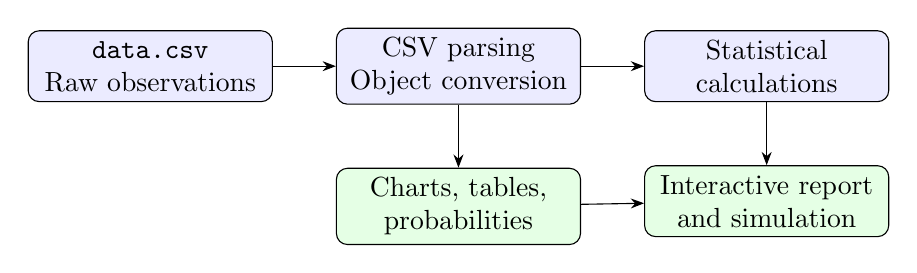
\begin{tikzpicture}[
    node distance=0.8cm,
    process/.style={draw, rounded corners, align=center, minimum width=3.1cm, minimum height=0.9cm, fill=blue!8},
    output/.style={draw, rounded corners, align=center, minimum width=3.1cm, minimum height=0.9cm, fill=green!10},
    >=Stealth
]
\node[process] (csv) {\texttt{data.csv}\\Raw observations};
\node[process, right=of csv] (parse) {CSV parsing\\Object conversion};
\node[process, right=of parse] (stats) {Statistical\\calculations};
\node[output, below=of parse] (charts) {Charts, tables,\\probabilities};
\node[output, below=of stats] (report) {Interactive report\\and simulation};
\draw[->] (csv) -- (parse);
\draw[->] (parse) -- (stats);
\draw[->] (stats) -- (report);
\draw[->] (parse) -- (charts);
\draw[->] (charts) -- (report);
\end{tikzpicture}
\caption{Image of the dashboard data processing workflow}
\label{fig:workflow-image}
\end{figure}

**Backend Architecture (Flask + Python)**:
The \texttt{app.py} Flask server implements all statistical computations using pandas, numpy, and scipy. The CSV dataset is loaded on startup into a pandas DataFrame. All computations (statistics, correlation, probability, hypothesis testing, simulation) are performed server-side and returned as JSON via RESTful API endpoints.

**Frontend Architecture (Vanilla JavaScript)**:
The \texttt{script.js} controls the data pipeline by making API calls to the Flask backend. The CSV file is retrieved and displayed via the \texttt{/api/load-data} endpoint, and all statistical calculations are fetched via specific API endpoints (\texttt{/api/statistics}, \texttt{/api/correlation}, \texttt{/api/probability}, \texttt{/api/hypothesis-test}, \texttt{/api/simulation}). The frontend handles table rendering, chart visualization, tab navigation, and DOM manipulation, but delegates all computational logic to Python.

The statistical section fetches mean, median, mode, variance, and standard deviation for the selected variable from the \texttt{/api/statistics/<column>} endpoint. The chart section uses Chart.js to visualize an appliance consumption line chart over time and a scatter plot of \texttt{Appliances} against \texttt{lights}. To improve performance, the charting code samples the dataset to a maximum of 650 plotted observations.

The inference section uses the \texttt{/api/probability} endpoint to compute empirical probabilities for user-selected thresholds. For example, the application estimates $P(\mathrm{Appliances} > t)$ for threshold values and $P(\mathrm{lights}=v)$ for lighting values. The hypothesis test is now dynamic: it uses the \texttt{/api/hypothesis-test} endpoint with two user-selected conditions:
\begin{itemize}
  \item Group 1: Appliance consumption where \texttt{lights} = [user-selected value] (e.g., 0, 30, 40, or 50 Wh)
  \item Group 2: Appliance consumption where \texttt{Appliances} $>$ [user-selected threshold] (e.g., 50, 100, 150, 200, or 250 Wh)
\end{itemize}
The backend performs an independent samples t-test comparing these two groups, returning the t-statistic, p-value, group means, standard deviations, and sample sizes. This allows users to explore different hypotheses interactively.

The simulation section generates random future-like values for \texttt{Appliances} or \texttt{lights}. The simulation uses the observed mean and standard deviation, combined with a user-selected noise level. The interface allows 10, 50, 100, or 500 simulations and displays the simulated mean, simulated variance, a line chart, and a results table.

\texttt{style.css} defines the visual presentation of the dashboard. It uses CSS custom properties for colors and spacing, responsive CSS Grid layouts for metric cards and charts, styled tables, tab controls, and print-oriented report styling. The design is responsive and adapts to desktop and smaller screen widths.


\section{Validation or Simulation (Reflection and
Critical Thinking)}
\label{sec:simulation}

**Validation and Correctness**:
The validation of the project is performed through consistency checks between the dataset, the Python backend computations, and the displayed dashboard values. The CSV contains 19,735 data rows and 29 columns. All statistical computations are performed by Python using pandas, numpy, and scipy, which are industry-standard libraries for numerical analysis. The key numerical results are verified against the dataset:

\begin{itemize}
  \item Appliance energy consumption: Mean = 97.695 Wh, Median = 60 Wh, Mode = 50 Wh, Std Dev = 102.522 Wh, Variance = 10,510.82 Wh²
  \item Range: 10–1,080 Wh (high variance reflects wide variability in household consumption patterns)
  \item Lights consumption: Mean = 3.80 Wh, with 77.28\% of observations at 0 Wh
  \item Correlation: Appliances vs Lights = 0.197 (weak positive relationship)
\end{itemize}

**Hypothesis Testing**:
The hypothesis test dynamically compares two user-selected groups using an independent samples t-test (scipy.stats.ttest\_ind). The test is flexible: users select which lighting level to compare (Group 1) and which appliance consumption threshold to compare (Group 2). The backend computes group statistics, t-statistic, and p-value to test whether the mean appliance consumption differs significantly between groups. Results include statistical significance at the 0.05 level.

**Simulation Component**:
The simulation component uses Monte Carlo methods with configurable noise levels (low 0.1$\sigma$, medium 0.3$\sigma$, high 0.5$\sigma$). It is not intended as a physical prediction model, but rather as a statistical experiment that uses the observed distribution to generate possible future values. This allows users to observe how variability assumptions affect simulated consumption patterns.

**Architecture Benefits**:
By implementing all computations in Python (Flask backend), the project ensures:
\begin{itemize}
  \item Accurate statistical computations using validated libraries (pandas, numpy, scipy)
  \item Scalability: the same backend can handle larger datasets without browser limitations
  \item Clarity: separation of concerns between frontend presentation and backend computation
  \item Reproducibility: statistical results are deterministic and independent of client-side JavaScript differences
\end{itemize}

\section{Conclusions}
\label{sec:conclusion}

**Summary of Findings**:
The project successfully applies statistical and probability concepts to a real household energy dataset through an interactive web dashboard. The analysis reveals that appliance energy consumption is highly variable (Std Dev = 102.522 Wh, nearly equal to the mean of 97.695 Wh), with observations ranging from 10 Wh to 1,080 Wh. This high variance reflects real household behavior: periods of baseline consumption (refrigerator, standby) interrupted by spikes when major appliances operate. The median value of 60 Wh is notably lower than the mean, indicating a right-skewed distribution where occasional high-consumption events pull the average upward.

Lighting consumption is frequently zero (77.28\% of observations), with a mean of only 3.80 Wh. The weak positive correlation (0.197) between appliance and lighting consumption suggests these variables are not strongly coupled—occupancy patterns influence both, but they operate somewhat independently.

**Technical Implementation**:
From an implementation perspective, the project demonstrates effective use of a Flask backend with Python statistical libraries (pandas, numpy, scipy) for computation, combined with a responsive frontend of HTML, CSS, and JavaScript using Chart.js for visualization. The dashboard integrates data loading, descriptive statistics, dynamic probability estimates, interactive hypothesis testing, visualization, Monte Carlo simulation, and report generation into a single web interface. The separation of computational logic (Python backend) from presentation logic (JavaScript frontend) ensures accuracy, scalability, and clarity.

**Educational Value**:
Overall, the work connects theoretical statistical methods taught in the course (descriptive statistics, correlation analysis, probability estimation, hypothesis testing, and simulation) with practical computational implementation. The interactive dashboard allows users to explore multiple hypotheses and experiment with different parameter selections, providing hands-on experience with statistical inference. This project demonstrates how statistical concepts become actionable insights when applied to real data with appropriate tools.

\newpage
\appendix

\section{Raw Data and Calculation Appendix}
\label{sec:appendix}

The complete raw dataset is retained with this report as the file \texttt{data.csv}. Since the file contains 19,735 observations and 29 variables, only a representative extract is printed in Table \ref{tab:raw-data-extract}. The calculations used for the main statistical conclusions are summarized in Table \ref{tab:calculation-summary}.

\begin{longtable}{|p{3.4cm}|p{1.6cm}|p{1.4cm}|p{1.5cm}|p{1.7cm}|p{1.6cm}|}
\caption{Raw data extract from \texttt{data.csv} using selected columns}
\label{tab:raw-data-extract}\\
\hline
\textbf{Date} & \textbf{Appliances} & \textbf{lights} & \textbf{T1} & \textbf{RH\_1} & \textbf{T\_out} \\
\hline
2016-01-11 17:00 & 60 & 30 & 19.890 & 47.597 & 6.600 \\
\hline
2016-01-11 17:10 & 60 & 30 & 19.890 & 46.693 & 6.483 \\
\hline
2016-01-11 17:20 & 50 & 30 & 19.890 & 46.300 & 6.367 \\
\hline
2016-01-11 17:30 & 50 & 40 & 19.890 & 46.067 & 6.250 \\
\hline
2016-01-11 17:40 & 60 & 40 & 19.890 & 46.333 & 6.133 \\
\hline
\end{longtable}

\begin{longtable}{|p{4cm}|p{9.2cm}|}
\caption{Calculation summary for reported statistical results}
\label{tab:calculation-summary}\\
\hline
\textbf{Calculation} & \textbf{Substitution and Result} \\
\hline
Total observations & $n = 19,735$ rows. \\
\hline
Mean appliance consumption & $\bar{x}_{A} = \frac{1,928,010}{19,735} = 97.695$ Wh. \\
\hline
Mean lighting consumption & $\bar{x}_{L} = \frac{75,030}{19,735} = 3.802$ Wh. \\
\hline
Appliance variance and standard deviation & $\sigma_A^2 = \frac{1}{19,735}\sum(x_i-97.695)^2 = 10,510.821$ and $\sigma_A=\sqrt{10,510.821}=102.522$ Wh. \\
\hline
Probability of high appliance use & $P(\mathrm{Appliances}>100)=\frac{4,233}{19,735}=0.2145=21.45\%$. \\
\hline
Probability of no lighting use & $P(\mathrm{lights}=0)=\frac{15,252}{19,735}=0.7728=77.28\%$. \\
\hline
Mean appliances when lights are 30 Wh & $\bar{x}_{30}=\frac{83,970}{559}=150.215$ Wh. \\
\hline
Mean appliances when lights are 40 or 50 Wh & $\bar{x}_{40,50}=\frac{15,650}{86}=181.977$ Wh. \\
\hline
Hypothesis comparison difference & $\bar{x}_{40,50}-\bar{x}_{30}=181.977-150.215=31.762$ Wh, indicating higher average appliance use in the higher-light group. \\
\hline
\end{longtable}

\end{document}